\documentclass{article}[18pt]
\usepackage{../../../../format}
\lhead{A Level Maths - M2}



\begin{document}
\begin{center}
\underline{\huge Statics of rigid bodies}
\end{center}
\section{Equilibrium of rigid bodies}
When calculating moments, only use the component of the force acting perpendicular to the rod.\\
\\
A rigid body is in equilibrium if:
\begin{itemize}
\item The vector sum of the forces is zero
\item The sum of the moments around any point is zero
\end{itemize}

If a rigid body is in equilibrium under the action of three non parallel forces, the lines of actions of the three forces all pass through the same point.\\
They can be arranged in a vector triangle to find forces

$$\textrm{Moment of a force about a point P}=|\textrm{Force}|\times\textrm{Perpendicular distance of the line of action of the force from the point P}$$
Essentially meaning, when taking non linear moments, the distances used should be the shortest distance from the point to where the force is acting.
\newpage
\begin{center}
\underline{\Huge Equilibrium of rigid bodies example}
\end{center}
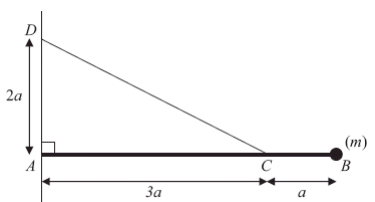
\includegraphics[width=8cm]{eq_rigid.png}\\
\textit{The diagram above shows a uniform rod AB of mass m and length 4a. The end A of the rod is
freely hinged to a point on a vertical wall. A particle of mass m is attached to the rod at B. One
end of a light inextensible string is attached to the rod at C, where AC = 3a. The other end of the
string is attached to the wall at D, where AD = 2a and D is vertically above A. The rod rests
horizontally in equilibrium in a vertical plane perpendicular to the wall and the tension in the
string is T. }\\
\\
\textit{Show that T = $mg\sqrt{13}$}\\
\\
Take moments about A 
$$3a\times T\cos\theta=2amg+4amg$$
Calculate $\cos\theta$ from the lengths on the diagram
$$\cos\theta=\frac{2}{\sqrt{3^2+2^2}}=\frac{2}{\sqrt{13}}$$
Substitute in the value of $\cos\theta$ and divide through by $a$
$$\frac{6}{\sqrt{13}}T=6mg$$
Multiply both sides by $\frac{\sqrt{13}}{6}$
$$T=mg\sqrt{13}$$
\\
\textit{The particle of mass m at B is removed from the rod and replaced by a particle of mass M which
is attached to the rod at B. The string breaks if the tension exceeds $2mg\sqrt{13}$. Given that the
string does not break,\\
show that $M\leqslant\frac{5}{2}m$}\\
\\
Rewrite the moments equation with the new information from the question
$$3a\times T\cos\theta=2amg+4aMg$$
Write the inequality given
$$T\leqslant 2mg\sqrt{13}$$
Substitute in the value for T
$$\frac{2mg+4Mg}{6}\sqrt{13}\leqslant2mg\sqrt{13}$$
Simplify
$$mg+2Mg\leqslant 6mg$$
$$M\leqslant\frac{5}{2}m$$
\end{document}